\section{Task 2.2 Image filtering and enhancement}

\subsection{Task 2.2.1}

Writing the partial derivatives on the form of eq 4.1 from the book will look
like so:
\begin{align}
  f(x,y) &=
    \sum_{i=I_\text{min}}^{I_\text{max}}
    \sum_{j=J_\text{min}}^{J_\text{max}} w(i,j)
    \frac{I(x+i+1,y+j) - I(x+i-1,y+j)}{2} \\
  f(x,y) &=
    \sum_{i=I_\text{min}}^{I_\text{max}}
    \sum_{j=J_\text{min}}^{J_\text{max}} w(i,j)
    \frac{I(x+i,y+j+1) - I(x+i,y+j-1)}{2}
\end{align}

I ran out of time before I could complete the rest of this task.

\subsection{Task 2.2.2}
I ran out of time before I could complete this task.

\subsection{Task 2.2.3}
The code for producing Figure \ref{fig:2_3_1} and the timings in Figure
\ref{fig:2_3_22} and Figure \ref{fig:2_3_21}, can be found in the appendix.
\graphicc{0.8}{img/2_3_1.png}{The image \textit{eight.tif} with different types
  of noise and filters.}{fig:2_3_1}

If the window size decides how big the kernel (and area of the image) is used to
calculate the pixel values.  Large windows sizes will thus tend to lower the
contrast of an image since all pixels take ``intensity cues'' from the other
pixels.

Figure \ref{fig:2_3_1} shows 2 different kinds of noise applied to the image
\textit{img/eight.tif}, and the result when applying different filters to the
noisy images. Figure \ref{fig:2_3_21} and \ref{fig:2_3_22} shows plots of the
time needed by each of the filters to run $100$ repetitions for different values
of $N$.

\begin{figure}
        \centering
        \begin{subfigure}[b]{0.9\textwidth}
                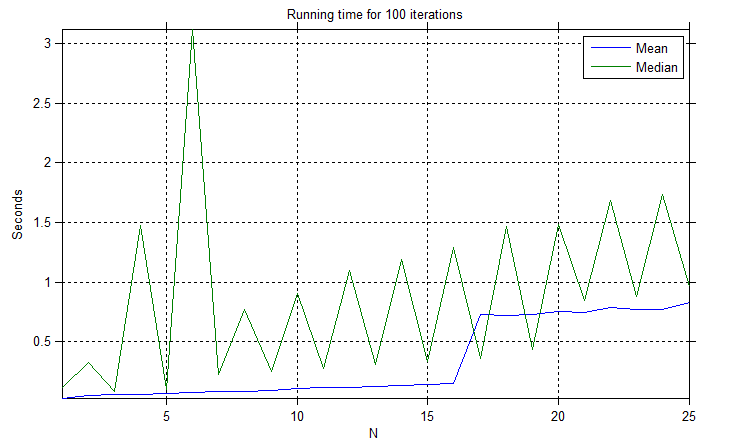
\includegraphics[width=\textwidth]{img/2_3_2.png}
                \caption{For $N \in [1,2,..,25]$.}
                \label{fig:2_3_21}
        \end{subfigure}%

        \begin{subfigure}[b]{0.9\textwidth}
                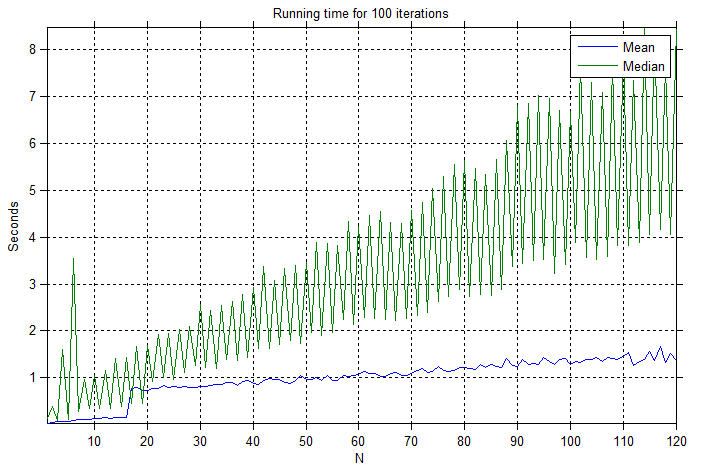
\includegraphics[width=\textwidth]{img/2_3_3.png}
                \caption{For $N \in [1,2,..,120]$.}
                \label{fig:2_3_22}
        \end{subfigure}
    \label{fig:2_3_2}
    \caption{}
\end{figure}

Figure \ref{fig:2_3_21} shows the running times for the specified number of
$N$. But because I found the initial spikes in the Median running time
suspicious I ran the test again, with $N$ values from $0$ to $120$, both to
better see how the running time evolves, and also to see if the high spike is a
pattern or singular. As seen on Figure \ref{fig:2_3_22} the spike is singular
for the beginning, but the constant increase/decrease cycle is a pattern for the
Median filter, albeit with an increase in amplitude and constant rise in running
time. The Mean filter shows much less variance and have pretty low running time
until $N \geq 17$ where it increases sharply and settles down again.



\subsection{Task 2.2.4}
The code for producing Figure \ref{fig:2_4} is found in the appendix. When $N$
increases over a certain threshold, the image no longer changes.  This happens
because even though we increase the window size, we do not increase the
$\sigma$-value, the weights around the center will decay to zero before reaching
the end of the window. Increasing sigma along with window size will yield
different results. As we shall see in the next section/task, increasing the
$\sigma$-value along with the window size will cause the image to blur more and
more.

\graphicc{0.8}{img/2_4.png}{The image \textit{eight.tif} with a Gaussian filter
  over it, using different values of $N$.}{fig:2_4}


\subsection{Task 2.2.5}
Code for producing Figure \ref{fig:2_5} can be found in the appendix.

Here I have tried different $\sigma$-values and increased the window size such
that $N = 3\times\sigma$.  The result, as mentioned above is that the image
blurs more and more until the shapes becomes undistinguishable.

\graphicc{0.9}{img/2_5.png}{Different $\sigma$-values and their impact on the
  filtering.}{fig:2_5}
